
\section{Superficies cuádricas}

\subsection{Definición y forma general}

Las superficies cuádricas son la extensión natural de las cónicas (elipse, parábola, hipérbola) al espacio tridimensional.

\begin{mydefinition}{Superficie cuádrica}
Una superficie cuádrica es el conjunto de puntos $(x, y, z) \in \mathbb{R}^3$ que satisfacen una ecuación de la forma:
\[
Ax^2 + By^2 + Cz^2 + Dxy + Exz + Fyz + Gx + Hy + Iz + J = 0
\]
donde $A, B, \ldots, J \in \mathbb{R}$ y al menos uno de los coeficientes cuadráticos es distinto de cero.
\end{mydefinition}

Aplicando traslaciones y rotaciones de los ejes, toda cuádrica no degenerada se reduce a una de las seis formas estándar que se estudian a continuación.

\subsection{Método de las trazas}

\begin{mydefinition}{Traza de una superficie}
La traza de una superficie en un plano $P$ es la curva de intersección entre ambos. Las trazas más útiles son:
\begin{itemize}
    \item $z = k$: intersección con un plano horizontal.
    \item $y = k$: intersección con un plano paralelo al plano $xz$.
    \item $x = k$: intersección con un plano paralelo al plano $yz$.
\end{itemize}
Al variar $k$, se observa cómo cambia la sección transversal, lo que permite reconstruir la forma tridimensional de la superficie.
\end{mydefinition}

\subsection{Elipsoide}

\begin{mydefinition}{Elipsoide}
La ecuación estándar del elipsoide centrado en el origen es:
\[
\frac{x^2}{a^2} + \frac{y^2}{b^2} + \frac{z^2}{c^2} = 1
\]
Los valores $a$, $b$ y $c$ son los semiejes en las direcciones $x$, $y$ y $z$ respectivamente. Si $a = b = c$, el elipsoide es una esfera de radio $a$.
\end{mydefinition}

\textbf{Trazas:} todas las trazas del elipsoide son elipses (o circunferencias en casos especiales).
\begin{itemize}
    \item $z = k$ (con $|k| < c$): $\;\dfrac{x^2}{a^2\left(1-\frac{k^2}{c^2}\right)} + \dfrac{y^2}{b^2\left(1-\frac{k^2}{c^2}\right)} = 1$ \quad (elipse)
    \item $y = 0$: $\;\dfrac{x^2}{a^2} + \dfrac{z^2}{c^2} = 1$ \quad (elipse en el plano $xz$)
    \item $x = 0$: $\;\dfrac{y^2}{b^2} + \dfrac{z^2}{c^2} = 1$ \quad (elipse en el plano $yz$)
\end{itemize}

El elipsoide es la única cuádrica acotada: todos sus puntos están dentro de la caja $[-a,a]\times[-b,b]\times[-c,c]$.

\begin{center}
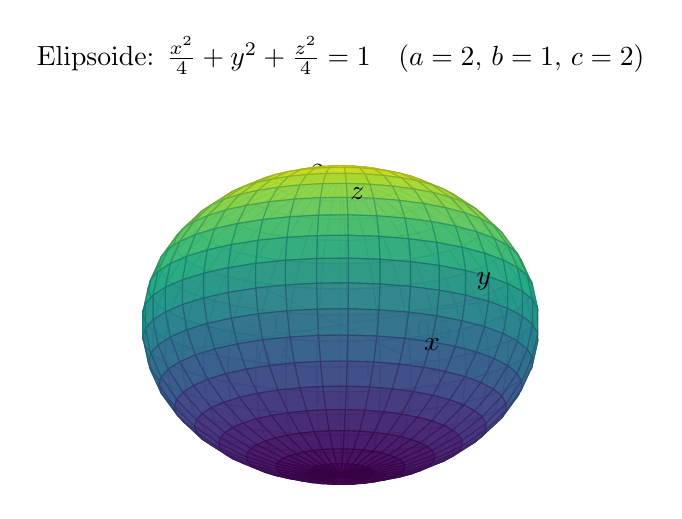
\begin{tikzpicture}
\begin{axis}[
    view={60}{20},
    axis lines=center,
    xlabel=$x$, ylabel=$y$, zlabel=$z$,
    colormap/viridis,
    title={Elipsoide: $\frac{x^2}{4} + y^2 + \frac{z^2}{4} = 1$\quad ($a=2,\,b=1,\,c=2$)}
]
\addplot3[
    surf,
    parametric,
    domain=0:360,
    domain y=0:180,
    samples=40,
    samples y=20,
    opacity=0.85
] ({2*sin(y)*cos(x)}, {sin(y)*sin(x)}, {2*cos(y)});
\end{axis}
\end{tikzpicture}
\end{center}

\subsection{Paraboloide elíptico}

\begin{mydefinition}{Paraboloide elíptico}
La ecuación estándar del paraboloide elíptico con vértice en el origen es:
\[
z = \frac{x^2}{a^2} + \frac{y^2}{b^2}
\]
La superficie se abre hacia el lado positivo del eje $z$. Si $a = b$, se obtiene el paraboloide circular (de revolución).
\end{mydefinition}

\textbf{Trazas:}
\begin{itemize}
    \item $z = k > 0$: $\;\dfrac{x^2}{a^2 k} + \dfrac{y^2}{b^2 k} = 1$ \quad (elipse que crece con $k$)
    \item $z = 0$: solo el vértice en el origen
    \item $y = 0$: $\;z = \dfrac{x^2}{a^2}$ \quad (parábola en el plano $xz$)
    \item $x = 0$: $\;z = \dfrac{y^2}{b^2}$ \quad (parábola en el plano $yz$)
\end{itemize}

\begin{center}
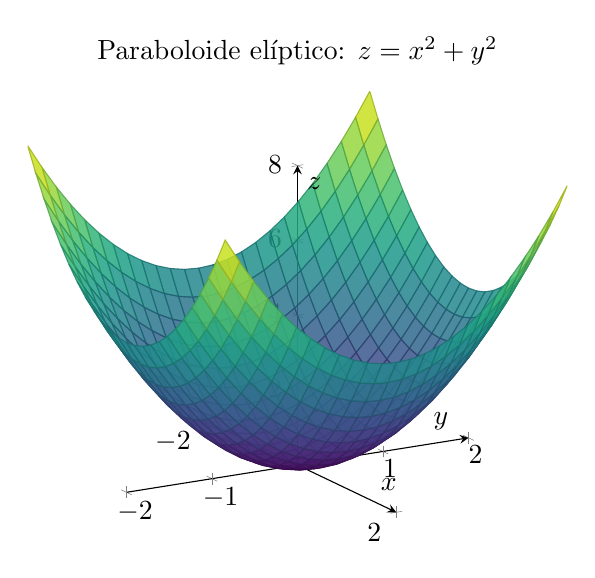
\begin{tikzpicture}
\begin{axis}[
    view={60}{20},
    axis lines=center,
    xlabel=$x$, ylabel=$y$, zlabel=$z$,
    colormap/viridis,
    zmin=0,
    title={Paraboloide elíptico: $z = x^2 + y^2$}
]
\addplot3[
    surf,
    domain=-2:2,
    domain y=-2:2,
    samples=25,
    opacity=0.85
] {x^2 + y^2};
\end{axis}
\end{tikzpicture}
\end{center}

\subsection{Paraboloide hiperbólico}

\begin{mydefinition}{Paraboloide hiperbólico}
La ecuación estándar del paraboloide hiperbólico con punto de silla en el origen es:
\[
z = \frac{y^2}{b^2} - \frac{x^2}{a^2}
\]
\end{mydefinition}

Esta superficie tiene la característica forma de silla de montar: desde el origen, sube en la dirección $y$ y baja en la dirección $x$.

\textbf{Trazas:}
\begin{itemize}
    \item $z = k > 0$: $\;\dfrac{y^2}{b^2 k} - \dfrac{x^2}{a^2 k} = 1$ \quad (hipérbola abierta en dirección $y$)
    \item $z = k < 0$: $\;\dfrac{x^2}{a^2|k|} - \dfrac{y^2}{b^2|k|} = 1$ \quad (hipérbola abierta en dirección $x$)
    \item $z = 0$: $\;y/b = \pm\, x/a$ \quad (dos rectas que se intersectan --- punto de silla)
    \item $y = 0$: $\;z = -\dfrac{x^2}{a^2}$ \quad (parábola hacia abajo)
    \item $x = 0$: $\;z = \dfrac{y^2}{b^2}$ \quad (parábola hacia arriba)
\end{itemize}

\begin{center}
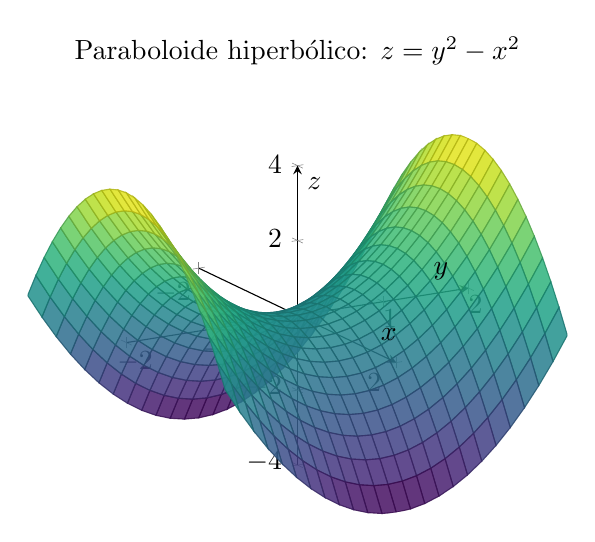
\begin{tikzpicture}
\begin{axis}[
    view={60}{20},
    axis lines=center,
    xlabel=$x$, ylabel=$y$, zlabel=$z$,
    colormap/viridis,
    title={Paraboloide hiperbólico: $z = y^2 - x^2$}
]
\addplot3[
    surf,
    domain=-2:2,
    domain y=-2:2,
    samples=25,
    opacity=0.85
] {y^2 - x^2};
\end{axis}
\end{tikzpicture}
\end{center}

\subsection{Cono elíptico}

\begin{mydefinition}{Cono elíptico}
La ecuación estándar del cono elíptico con vértice en el origen es:
\[
\frac{x^2}{a^2} + \frac{y^2}{b^2} = \frac{z^2}{c^2}
\]
Cuando $a = b$, se obtiene el cono circular recto. La superficie consta de dos napas simétricas respecto al origen.
\end{mydefinition}

\textbf{Trazas:}
\begin{itemize}
    \item $z = k \neq 0$: $\;\dfrac{x^2}{\left(\frac{ak}{c}\right)^2} + \dfrac{y^2}{\left(\frac{bk}{c}\right)^2} = 1$ \quad (elipse que se expande con $|k|$)
    \item $z = 0$: solo el vértice en el origen
    \item $y = 0$: $\;z = \pm\,\dfrac{c}{a}x$ \quad (dos rectas que se cruzan)
    \item $x = 0$: $\;z = \pm\,\dfrac{c}{b}y$ \quad (dos rectas que se cruzan)
\end{itemize}

\begin{center}
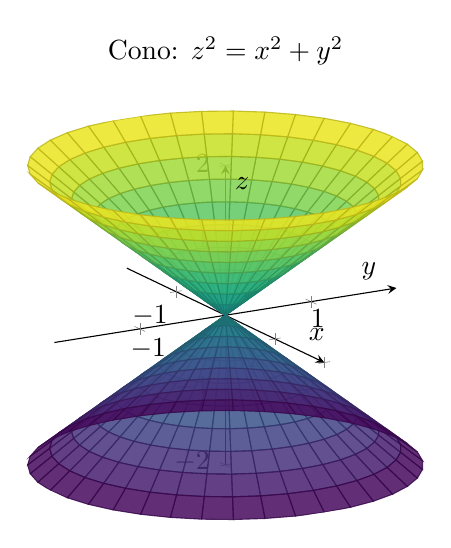
\begin{tikzpicture}
\begin{axis}[
    view={60}{20},
    axis lines=center,
    xlabel=$x$, ylabel=$y$, zlabel=$z$,
    colormap/viridis,
    title={Cono: $z^2 = x^2 + y^2$}
]
\addplot3[
    surf,
    parametric,
    domain=0:360,
    domain y=0:2,
    samples=40,
    samples y=10,
    opacity=0.85
] ({y*cos(x)}, {y*sin(x)}, {y});
\addplot3[
    surf,
    parametric,
    domain=0:360,
    domain y=0:2,
    samples=40,
    samples y=10,
    opacity=0.85
] ({y*cos(x)}, {y*sin(x)}, {-y});
\end{axis}
\end{tikzpicture}
\end{center}

\subsection{Hiperboloide de una hoja}

\begin{mydefinition}{Hiperboloide de una hoja}
La ecuación estándar del hiperboloide de una hoja con eje a lo largo de $z$ es:
\[
\frac{x^2}{a^2} + \frac{y^2}{b^2} - \frac{z^2}{c^2} = 1
\]
\end{mydefinition}

El hiperboloide de una hoja es una superficie conexa (una sola pieza). Su sección transversal horizontal es siempre una elipse, con tamaño mínimo en $z = 0$ que crece conforme $|z|$ aumenta.

\textbf{Trazas:}
\begin{itemize}
    \item $z = k$: $\;\dfrac{x^2}{a^2\left(1+\frac{k^2}{c^2}\right)} + \dfrac{y^2}{b^2\left(1+\frac{k^2}{c^2}\right)} = 1$ \quad (elipse mínima en $k=0$)
    \item $y = 0$: $\;\dfrac{x^2}{a^2} - \dfrac{z^2}{c^2} = 1$ \quad (hipérbola)
    \item $x = 0$: $\;\dfrac{y^2}{b^2} - \dfrac{z^2}{c^2} = 1$ \quad (hipérbola)
\end{itemize}

\begin{mynote}{Relación con el cono}
El cono y el hiperboloide de una hoja solo difieren en el lado derecho de la expresión $\dfrac{x^2}{a^2}+\dfrac{y^2}{b^2}-\dfrac{z^2}{c^2}$: es $0$ para el cono y $1$ para el hiperboloide. Las ``paredes'' del hiperboloide se acercan asintóticamente al cono cuando $|z|\to\infty$.
\end{mynote}

\begin{center}
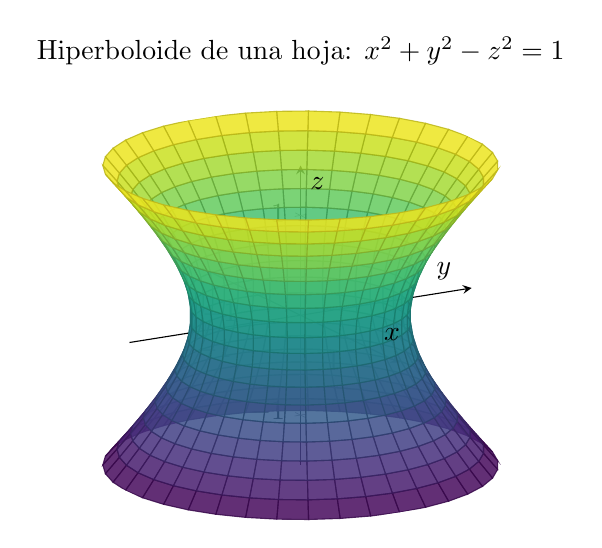
\begin{tikzpicture}
\begin{axis}[
    view={60}{20},
    axis lines=center,
    xlabel=$x$, ylabel=$y$, zlabel=$z$,
    colormap/viridis,
    title={Hiperboloide de una hoja: $x^2 + y^2 - z^2 = 1$}
]
\addplot3[
    surf,
    parametric,
    domain=0:360,
    domain y=-1.5:1.5,
    samples=40,
    samples y=20,
    opacity=0.85
] ({sqrt(1+y^2)*cos(x)}, {sqrt(1+y^2)*sin(x)}, {y});
\end{axis}
\end{tikzpicture}
\end{center}

\subsection{Hiperboloide de dos hojas}

\begin{mydefinition}{Hiperboloide de dos hojas}
La ecuación estándar del hiperboloide de dos hojas con eje a lo largo de $z$ es:
\[
\frac{z^2}{c^2} - \frac{x^2}{a^2} - \frac{y^2}{b^2} = 1
\]
\end{mydefinition}

Para que la ecuación tenga solución real se requiere $z^2/c^2 \geq 1$, es decir, $|z| \geq c$. La superficie no existe en la región $-c < z < c$ y consta de dos componentes separadas: una hoja para $z \geq c$ y otra para $z \leq -c$.

\textbf{Trazas:}
\begin{itemize}
    \item $z = k$ con $|k| > c$: $\;\dfrac{x^2}{a^2\!\left(\frac{k^2}{c^2}-1\right)} + \dfrac{y^2}{b^2\!\left(\frac{k^2}{c^2}-1\right)} = 1$ \quad (elipse)
    \item $|z| < c$: no existe traza (región vacía)
    \item $y = 0$: $\;\dfrac{z^2}{c^2} - \dfrac{x^2}{a^2} = 1$ \quad (hipérbola abierta en dirección $z$)
    \item $x = 0$: $\;\dfrac{z^2}{c^2} - \dfrac{y^2}{b^2} = 1$ \quad (hipérbola abierta en dirección $z$)
\end{itemize}

\begin{center}
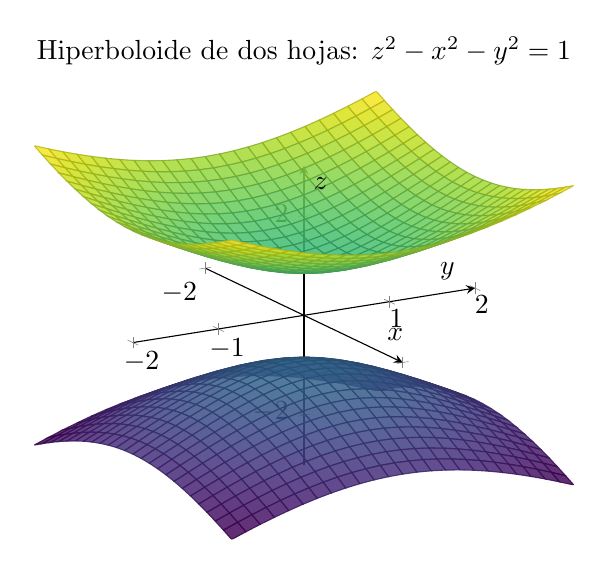
\begin{tikzpicture}
\begin{axis}[
    view={60}{20},
    axis lines=center,
    xlabel=$x$, ylabel=$y$, zlabel=$z$,
    colormap/viridis,
    title={Hiperboloide de dos hojas: $z^2 - x^2 - y^2 = 1$}
]
\addplot3[
    surf,
    domain=-2:2,
    domain y=-2:2,
    samples=25,
    opacity=0.85
] {sqrt(1+x^2+y^2)};
\addplot3[
    surf,
    domain=-2:2,
    domain y=-2:2,
    samples=25,
    opacity=0.85
] {-sqrt(1+x^2+y^2)};
\end{axis}
\end{tikzpicture}
\end{center}

\subsection{Resumen de superficies cuádricas}

\begin{center}
\renewcommand{\arraystretch}{2.2}
\begin{tabular}{|l|c|l|}
\hline
\textbf{Superficie} & \textbf{Ecuación estándar (eje $z$)} & \textbf{Trazas características} \\
\hline
Elipsoide & $\dfrac{x^2}{a^2}+\dfrac{y^2}{b^2}+\dfrac{z^2}{c^2}=1$ & Todas elipses \\
\hline
Paraboloide elíptico & $z=\dfrac{x^2}{a^2}+\dfrac{y^2}{b^2}$ & Elipses (horiz.) / Parábolas (vert.) \\
\hline
Paraboloide hiperbólico & $z=\dfrac{y^2}{b^2}-\dfrac{x^2}{a^2}$ & Hipérbolas / Parábolas \\
\hline
Cono elíptico & $\dfrac{x^2}{a^2}+\dfrac{y^2}{b^2}=\dfrac{z^2}{c^2}$ & Elipses / Rectas cruzadas \\
\hline
Hiperboloide de una hoja & $\dfrac{x^2}{a^2}+\dfrac{y^2}{b^2}-\dfrac{z^2}{c^2}=1$ & Elipses / Hipérbolas \\
\hline
Hiperboloide de dos hojas & $\dfrac{z^2}{c^2}-\dfrac{x^2}{a^2}-\dfrac{y^2}{b^2}=1$ & Elipses (si $|z|>c$) / Hipérbolas \\
\hline
\end{tabular}
\end{center}


\subsection{Ejercicios}

\begin{enumerate}
    \item Identificar el tipo de superficie cuádrica de cada ecuación (elipsoide, paraboloide elíptico, paraboloide hiperbólico, cono, hiperboloide de una hoja o hiperboloide de dos hojas). Justificar la clasificación.
\begin{enumerate}
    \item $\dfrac{x^2}{4} + \dfrac{y^2}{9} + \dfrac{z^2}{1} = 1$
    \item $z = x^2 + 4y^2$
    \item $x^2 + y^2 - z^2 = 1$
    \item $\dfrac{x^2}{4} + \dfrac{y^2}{9} - \dfrac{z^2}{16} = 0$
    \item $z^2 - x^2 - y^2 = 4$
    \item $z = y^2 - x^2$
\end{enumerate}
    \item Completar el cuadrado en las variables correspondientes para llevar cada ecuación a su forma estándar. Identificar el tipo de cuádrica, el centro y los semiejes o vértice según corresponda.
\begin{enumerate}
    \item $4x^2 + y^2 + 9z^2 - 8x + 2y - 36z + 37 = 0$
    \item $z = x^2 - 4x + y^2 + 6y + 13$
    \item $x^2 + y^2 - z^2 - 2x + 4y + 2z - 2 = 0$
\end{enumerate}

\textit{Sugerencia:} Para el inciso (a), completar el cuadrado en $x$, $y$ y $z$ por separado y verificar si el lado derecho resulta positivo.
    \item Para el elipsoide $\dfrac{x^2}{9} + \dfrac{y^2}{4} + \dfrac{z^2}{16} = 1$:
\begin{enumerate}
    \item Identificar los semiejes $a$, $b$ y $c$ en las direcciones $x$, $y$ y $z$.
    \item Encontrar las trazas con los tres planos coordenados ($z=0$, $y=0$, $x=0$) y describir cada cónica obtenida.
    \item Encontrar la traza con el plano $z = 2$ y determinar sus semiejes.
    \item Determinar si los puntos $P_1 = (3, 0, 0)$, $P_2 = (1, 1, 2)$ y $P_3 = (0, 2, 4)$ están sobre, dentro o fuera del elipsoide.
    \item ¿Para qué valores de $k$ el plano $z = k$ interseca al elipsoide?
\end{enumerate}
    \item El paraboloide elíptico $z = \dfrac{x^2}{4} + \dfrac{y^2}{9}$ tiene su vértice en el origen.
\begin{enumerate}
    \item Encontrar la traza con el plano $z = 1$ y calcular el área de la elipse obtenida usando $A = \pi ab$.
    \item Encontrar las trazas con los planos $y = 0$ y $x = 0$. ¿Qué tipo de curva es cada una?
    \item Determinar el punto de la superficie más cercano al origen. ¿Cuál es ese punto?
    \item El plano $z = 4$ corta al paraboloide. Encontrar la ecuación de la elipse de intersección y calcular su área.
    \item Describir cómo cambia la forma de las trazas horizontales $z = k$ al aumentar $k$ desde $0$ hasta $\infty$.
\end{enumerate}
    \item El paraboloide hiperbólico $z = x^2 - y^2$ tiene un punto de silla en el origen.
\begin{enumerate}
    \item Encontrar las trazas con los planos $z = 1$, $z = -1$ y $z = 0$, e identificar las cónicas obtenidas.
    \item Las trazas con $y = 0$ y $x = 0$ son parábolas. Determinar en qué dirección se abren.
    \item Verificar que el origen es un punto de silla: mostrar que a lo largo de la dirección $x$ el origen es un mínimo local de $z$, y a lo largo de la dirección $y$ es un máximo local.
    \item Encontrar todos los puntos de la superficie con $z = 0$ (la curva del ``ecuador'' de la silla). ¿Qué rectas son estas?
    \item Determinar si el punto $P = (3, 2, 5)$ pertenece a la superficie.
\end{enumerate}
    \item Dado el cono elíptico $\dfrac{x^2}{4} + \dfrac{y^2}{9} = z^2$:
\begin{enumerate}
    \item Verificar que el vértice se encuentra en el origen.
    \item Encontrar las trazas con los planos $z = 1$, $z = 2$ y $z = -1$. Identificar qué tipo de curva es cada una e indicar los semiejes.
    \item Encontrar las trazas con $y = 0$ y $x = 0$ y mostrar que son pares de rectas.
    \item ¿Cuántas napas (mitades) tiene el cono? Describir la napa superior ($z > 0$) y la inferior ($z < 0$).
    \item El plano $z = k$ interseca al cono en una elipse para todo $k \neq 0$. Escribir la fórmula de los semiejes en función de $k$ y calcular el área de la sección transversal.
\end{enumerate}
    \item Para el hiperboloide de una hoja $\dfrac{x^2}{4} + \dfrac{y^2}{4} - \dfrac{z^2}{9} = 1$:
\begin{enumerate}
    \item Identificar los semiejes $a$, $b$, $c$ y describir la orientación de la superficie.
    \item Encontrar la traza con $z = 0$ (la ``cintura'' del hiperboloide) e identificar su tipo y radio.
    \item Encontrar la traza con $z = 3$ y comparar su tamaño con la traza en $z = 0$.
    \item Encontrar las trazas con $y = 0$ y $x = 0$. ¿Qué tipo de cónica es cada una?
    \item Determinar para qué valores de $k$ el plano $z = k$ produce una traza válida (es decir, siempre existe intersección). Comparar con el hiperboloide de dos hojas.
\end{enumerate}
    \item Para el hiperboloide de dos hojas $\dfrac{z^2}{4} - \dfrac{x^2}{9} - \dfrac{y^2}{9} = 1$:
\begin{enumerate}
    \item Determinar los valores de $z$ para los cuales existe la superficie. ¿Cuál es la región vacía?
    \item Encontrar los vértices del hiperboloide (los puntos de las hojas más cercanos al origen).
    \item Encontrar la traza con el plano $z = 4$ e identificar su tipo y semiejes.
    \item Encontrar las trazas con $y = 0$ y $x = 0$. ¿Qué hipérbolas se obtienen?
    \item Comparar las ecuaciones del hiperboloide de una hoja y del de dos hojas del ejercicio anterior. ¿Qué diferencia hay en los signos? ¿Cómo afecta esto a la topología (número de componentes conexas)?
\end{enumerate}
    \item Una superficie cuádrica tiene la ecuación general:
\[
9x^2 + 4y^2 - 36z^2 - 18x + 16y + 72z - 11 = 0
\]

\begin{enumerate}
    \item Completar el cuadrado en cada variable para llevar la ecuación a su forma estándar.
    \item Identificar el tipo de superficie cuádrica e indicar el centro.
    \item Encontrar los semiejes de la superficie.
    \item Describir las trazas con cada plano coordenado trasladado al nuevo centro.
\end{enumerate}

\textit{Sugerencia:} Agrupar los términos en $x$, en $y$ y en $z$ por separado antes de completar el cuadrado.
    \item Encontrar la ecuación de la superficie cuádrica que satisface cada descripción. Escribir la ecuación en forma estándar.
\begin{enumerate}
    \item \textbf{Elipsoide} centrado en el origen que pasa por los puntos $(4, 0, 0)$, $(0, 2, 0)$ y $(0, 0, 3)$.
    \item \textbf{Paraboloide elíptico} con vértice en el origen, eje a lo largo de $z$ positivo, que pasa por el punto $(2, 1, 2)$.
    \item \textbf{Cono circular} con vértice en el origen y eje a lo largo de $z$, tal que la traza con el plano $z = 1$ es la circunferencia $x^2 + y^2 = 3$.
    \item \textbf{Hiperboloide de una hoja} con eje a lo largo de $z$, semiejes horizontales $a = b = 2$ y tal que la traza con $z = 2$ tenga semiejes $a' = b' = 2\sqrt{2}$.
    \item \textbf{Hiperboloide de dos hojas} con eje a lo largo de $z$ y vértices en $(0, 0, \pm 3)$, con semiejes horizontales $a = b = 2$.
\end{enumerate}
\end{enumerate}
